\section{Auditive \& Visuelle Systeme}
\subsection{Auditives System}
Das auditive System nimmt Schallereignisse wahr und vermittelt diese an das Gehirn. Es teilt sich dabei in peripheres und zentrales auditives System, welche je Aufnahme und Vermittlung übernehmen.

Das periphere auditive System umfasst die anatomischen Strukturen, die zur Wahrnehmung der Druckschwankungen dienen. Diese werden wiederum in Außenohr, Mittelohr und Innenohr unterteilt.

\begin{figure}[H]
	\centering
	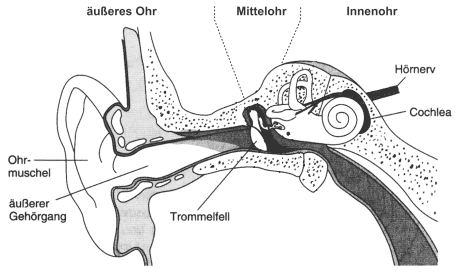
\includegraphics[height=5cm]{images/auditive-system.png}
	\caption{Auditives System am Menschen \cite{netaudio:as}}
	\label{fig:as}
\end{figure}

Das zentrale auditive System beinhaltet den Hörnerv, welcher die Signale des peripheren Systems übermittelt, sowie Regionen des Gehirns, welche diese Informationen auditiv verarbeiten. Es wird hier thematisch bedingt nicht behandelt.

\subsubsection{Außenohr}
\begin{wrapfigure}{R}{.45\textwidth}
 	\centering
 	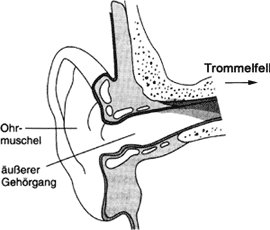
\includegraphics[height=4cm]{images/aussenohr.png}
	\caption{Außenohr am Menschen \cite{netaudio:aussenohr}}
	\label{fig:aussenohr}
\end{wrapfigure}

Das Außenohr umfasst die Ohrmuschel, sowie den äußeren Gehörgang. Am Menschen ist sie ein nahezu funktionsloses Relikt der Evolution, während sie bei den meisten Säugetieren aktiv bewegt werden kann und zur Schallortung eingesetzt wird.

Der Gehörgang dient zum Schutz der Sinnesorgane im Innenohr und optimiert zudem durch Resonanzeffekte das Hören von Information. Damit wird unter anderem die Sprachverständlichkeit verbessert, indem die wichtigen Frequenzanteile zwischen 2 und 4 \gls{ac:khz} hervorgehoben werden.

\newpage
\subsubsection{Mittelohr}
\enquote{Am Ende des äußeren Gehörgangs liegt das Trommelfell. Diese Membran überträgt die Schwingungen der Luft auf die Knochenstrukturen des Mittelohrs.}
~\-- NetAudio,~\citeyear{netaudio:mittelohr}~\cite{netaudio:mittelohr}

\begin{wrapfigure}{R}{.52\textwidth}
	\centering
	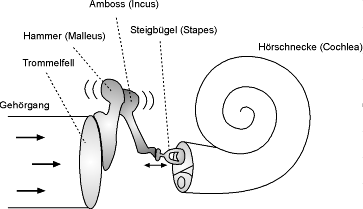
\includegraphics[height=4cm]{images/ossikel.png}
	\caption{Knöchelchen im Mittelohr \cite{netaudio:mittelohr}}
	\label{fig:ossikel}
\end{wrapfigure}

~\\
Im Mittelohr befinden sich drei miteinander verbundene Knöchelchen, welche als Ossikel bezeichnet werden. Direkt am Trommelfell befindet sich der Hammer (Malleus), der Schwingungen an Amboss (Incus) und Steigbügel (Stapes) weitergibt.

Der Steigbügel sitzt dabei auf einer Membran, die eine Öffnung zum Innenohr abdeckt, und leitet so durch seine Bewegung, Schwingungen an die Hörschnecke (Cochlea) weiter.

\subsubsection{Innenohr}
Den wichtigsten Teil des Innenohrs bildet die Hörschnecke (Cochlea), welche in obiger Abbildung \ref{fig:ossikel} rechts zu sehen ist.

In der Hörschnecke befindet sich zwischen zwei Membranen (Basilarmembran und Tektorialmembran), das eigentliche Sinnesorgan, das Cortische Organ. Die Druckwellen in der Hörschnecke eine Wellenbewegung auf der Basilarmembran aus. Kleinste Haarzellen am Cortischen Organ, reiben an der Oberfläche der Tektorialmembran und veranlassen eine Ausschüttung chemischer Botenstoffe, welche wiederum Signale an das zentrale auditive System weiterleiten.


% TODO: \subsection{Visuelles System}
